\documentclass[12pt,a4paper]{article}
\usepackage{fontspec}
\setmainfont{Latin Modern Roman}
\setmonofont{DejaVu Sans Mono}[Scale=0.77]
\usepackage[a4paper,left=27mm,right=22mm,top=23mm,bottom=23mm]{geometry}
\usepackage{amsmath,amssymb,graphicx,booktabs,tabularx,array,longtable,float,enumitem,setspace,fancyhdr,titlesec,caption,listings,xcolor,hyperref}
\usepackage{tikz}
\definecolor{CoverBlue}{HTML}{0078B8}
\setlength{\arrayrulewidth}{0.45pt}
\setstretch{1.15}
\setlength{\parskip}{3pt}
\setlength{\parindent}{6mm}
\setlength{\headheight}{15pt}
\setlength{\emergencystretch}{3em}
\setlist{nosep,topsep=4pt,leftmargin=1.7em}
\newcolumntype{Y}{>{\raggedright\arraybackslash}X}
\hypersetup{hidelinks,pdftitle={Bloxorz Solver},pdfauthor={Huỳnh Thanh Huy; Hồ Hữu Nghiêm; Chu Bảo Minh; Trần Thị Bích Hạnh; Võ Trúc Quỳnh}}
\fancyhf{}
\fancyhead[L]{\small CSC14003}
\fancyhead[R]{\small Bloxorz Solver}
\fancyfoot[C]{\thepage}
\renewcommand{\headrulewidth}{0.3pt}
\titleformat{\section}{\large\bfseries}{\thesection}{0.7em}{}
\titleformat{\subsection}{\normalsize\bfseries}{\thesubsection}{0.7em}{}
\titleformat{\subsubsection}{\normalsize\bfseries\itshape}{\thesubsubsection}{0.7em}{}
\titlespacing*{\section}{0pt}{12pt}{6pt}
\titlespacing*{\subsection}{0pt}{9pt}{4pt}
\captionsetup{font=small,labelfont=bf,skip=5pt}
\renewcommand{\contentsname}{Mục lục}
\renewcommand{\tablename}{Bảng}
\renewcommand{\figurename}{Hình}
\renewcommand{\refname}{Tài liệu tham khảo}
\lstset{basicstyle=\ttfamily\small,breaklines=true,columns=fullflexible,frame=single,rulecolor=\color{black!25},numbers=none,aboveskip=8pt,belowskip=8pt,showstringspaces=false}
\renewcommand{\lstlistingname}{Mã giả}
\newcommand{\hinhanh}[3][0.95\linewidth]{\begin{figure}[htbp]\centering\includegraphics[width=#1]{figures/#2}\caption{#3}\end{figure}}
\setcounter{tocdepth}{2}
\begin{document}
\begin{titlepage}
\begin{tikzpicture}[remember picture,overlay]
\draw[CoverBlue,line width=1.6pt] ([xshift=14mm,yshift=-14mm]current page.north west) rectangle ([xshift=-14mm,yshift=14mm]current page.south east);
\draw[CoverBlue!65,line width=0.5pt] ([xshift=16mm,yshift=-16mm]current page.north west) rectangle ([xshift=-16mm,yshift=16mm]current page.south east);
\end{tikzpicture}
\centering
{\bfseries ĐẠI HỌC QUỐC GIA THÀNH PHỐ HỒ CHÍ MINH\par}
{\bfseries TRƯỜNG ĐẠI HỌC KHOA HỌC TỰ NHIÊN\par}
{KHOA CÔNG NGHỆ THÔNG TIN\par}
\vspace{18mm}

\includegraphics[width=50mm]{figures/hcmus_logo.png}
\vspace{13mm}

{\large\bfseries BÁO CÁO ĐỒ ÁN 1\par}
\vspace{6mm}
{\Huge\bfseries BLOXORZ SOLVER\par}
\vspace{8mm}
{\large Nhập môn Trí tuệ nhân tạo\par}
{Mã học phần CSC14003\par}
\vspace{12mm}
{\bfseries GIẢNG VIÊN HƯỚNG DẪN\par}
GV. Nguyễn Thanh Tình\par
\vspace{12mm}
{\bfseries NHÓM THỰC HIỆN : 8\par}
\vspace{5mm}
\renewcommand{\arraystretch}{1.3}
\begin{tabular}{ll}
MSSV & Họ và tên\\
24120323 & Huỳnh Thanh Huy\\
24120390 & Hồ Hữu Nghiêm\\
24120379 & Chu Bảo Minh\\
24120304 & Trần Thị Bích Hạnh\\
24120427 & Võ Trúc Quỳnh
\end{tabular}
\vfill
Thành phố Hồ Chí Minh, ngày 1 tháng 11 năm 2026
\end{titlepage}
\pagestyle{fancy}
\pagenumbering{arabic}
{\small\setstretch{1.0}\setlength{\parskip}{0pt}\tableofcontents}
\clearpage
\section{Tổng quan và kế hoạch thực hiện}
\subsection{Giới thiệu bài toán}
Bloxorz là trò chơi điều khiển một khối hộp kích thước $1\times1\times2$ trên bàn ô vuông. Người chơi lăn khối theo bốn hướng để đưa khối đứng thẳng vào ô đích. Khó khăn nằm ở việc vị trí và tư thế của khối cùng quyết định nước đi hợp lệ: khi đứng, khối chiếm một ô; khi nằm, khối chiếm hai ô. Các ô dễ vỡ, công tắc, cầu và cơ chế tách khối làm trạng thái bài toán thay đổi theo lịch sử di chuyển.

Đồ án xây dựng trò chơi có giao diện và bốn bộ giải BFS, DFS, UCS, A*. Mục tiêu không chỉ là tìm một lời giải mà còn so sánh chất lượng lời giải và tài nguyên tìm kiếm trên cùng bộ màn chơi, theo yêu cầu trong đề bài~\cite{de}.

\subsection{Mục tiêu và phạm vi}
Chương trình được viết bằng Python, sử dụng Ursina cho giao diện. Nhóm tự cài đặt các thuật toán tìm kiếm; các cấu trúc như danh sách, tập hợp, từ điển và hàng đợi ưu tiên chỉ đóng vai trò hỗ trợ. Màn chơi được mô tả bằng JSON để dùng chung giữa chơi tay, giải tự động và thực nghiệm.

Phạm vi chức năng gồm: các phép lăn cơ bản; kiểm tra rơi và thắng; fragile, bridge, soft switch, heavy switch, split switch; điều khiển từng cube sau khi tách; phát lại lời giải; ghi nhận thời gian, bộ nhớ, số nút mở rộng, số hành động và tổng chi phí. Báo cáo phân biệt số hành động với chi phí, vì hai đại lượng này không tương đương khi sử dụng trọng số $1$--$2$--$4$.



\subsection{Kế hoạch và phân công}

Nhóm gồm năm thành viên, phối hợp xây dựng trò chơi,
cài đặt bốn thuật toán tìm kiếm, thực hiện thực nghiệm,
viết báo cáo và quay video minh họa. Quy trình thực hiện gồm xây dựng luật chơi, tích hợp bộ giải, đo thực nghiệm và tổng hợp kết quả.

\begin{table}[htbp]
\centering
\small
\caption{Phân công nhiệm vụ và mức độ hoàn thành}
\begin{tabularx}{\linewidth}{|p{3.8cm}|X|c|}
\hline
\textbf{Thành viên}
& \textbf{Nhiệm vụ}
& \textbf{Hoàn thành} \\\hline
Huỳnh Thanh Huy \newline 24120323
& Xây dựng trò chơi cùng Chu Bảo Minh;
  cài đặt thuật toán BFS.
& 100\% \\\hline
Hồ Hữu Nghiêm \newline 24120390
& Cài đặt thuật toán UCS;
  viết phần mô tả các thuật toán trong báo cáo.
& 100\% \\\hline
Chu Bảo Minh \newline 24120379
& Xây dựng trò chơi cùng Huỳnh Thanh Huy;
  thực hiện video demo.
& 100\% \\\hline
Trần Thị Bích Hạnh \newline 24120304
& Cài đặt thuật toán A*;
  thực hiện và trình bày phần thực nghiệm
  cùng Võ Trúc Quỳnh.
& 100\% \\\hline
Võ Trúc Quỳnh \newline 24120427
& Cài đặt thuật toán DFS;
  thực hiện và trình bày phần thực nghiệm
  cùng Trần Thị Bích Hạnh.
& 100\% \\\hline
\end{tabularx}
\end{table}

Theo đánh giá của nhóm, mỗi thành viên hoàn thành
100\% nhiệm vụ được phân công. Tỷ lệ này thể hiện
mức độ hoàn thành nhiệm vụ của từng thành viên,
không phải tỷ lệ đóng góp cộng lại của cả nhóm.


\section{Mô hình hóa bài toán tìm kiếm}
\subsection{Bản đồ và trạng thái}
Bản đồ là lưới hữu hạn với kích thước $H\times W$. Thông tin tĩnh gồm loại ô, vị trí đích, nhóm cầu, liên kết công tắc và các vị trí teleport. Thông tin động được lưu trong \texttt{GameState}, có thể biểu diễn:
\[
s=(b,\boldsymbol{\beta},C,a).
\]
Trong đó $b=(r,c,o)$ mô tả khối và tư thế $o$; $\boldsymbol{\beta}$ là bộ giá trị đóng/mở của các nhóm cầu; $C$ là vị trí hai cube khi tách, rỗng khi chưa tách; $a$ là cube đang điều khiển hoặc giá trị rỗng khi khối đã ghép.

\begin{table}[htbp]\centering
\caption{Các tư thế và ô bị chiếm}
\begin{tabularx}{\linewidth}{|l|Y|}
\hline Tư thế & Các ô bị chiếm\\\hline
\texttt{STANDING} & $(r,c)$\\\hline
\texttt{HORIZONTAL} & $(r,c)$ và $(r,c+1)$\\\hline
\texttt{VERTICAL} & $(r,c)$ và $(r+1,c)$\\\hline
\texttt{CUBE} & Khi tách, dùng hai tọa độ trong $C$; $b$ theo cube chủ động.\\\hline
\end{tabularx}
\end{table}
Hai trạng thái chỉ bằng nhau khi các thành phần động tương ứng bằng nhau. Đặc biệt, cùng vị trí khối nhưng khác cấu hình cầu là hai trạng thái khác nhau. Kiểu dữ liệu bất biến và hàm băm cho phép dùng trạng thái làm phần tử của \texttt{visited} hoặc khóa của \texttt{parents}, \texttt{best\_cost}.

\subsection{Hành động và chuyển trạng thái}
Khối chưa tách có bốn hành động \texttt{UP}, \texttt{DOWN}, \texttt{LEFT}, \texttt{RIGHT}. Khi tách, mỗi hướng di chuyển cube chủ động một ô; \texttt{SWITCH} đổi cube đang điều khiển mà không thay đổi vị trí. Trong cách đếm hiện tại, \texttt{SWITCH} cũng là một hành động.

\begin{table}[htbp]\centering\small
\caption{Bảng chuyển tư thế của khối lớn; tọa độ là ô neo của tư thế mới}
\begin{tabular}{|l|l|l|l|l|}
\hline Tư thế & Up & Down & Left & Right\\\hline
Đứng & $(r-2,c,V)$ & $(r+1,c,V)$ & $(r,c-2,H)$ & $(r,c+1,H)$\\\hline
Nằm ngang & $(r-1,c,H)$ & $(r+1,c,H)$ & $(r,c-1,S)$ & $(r,c+2,S)$\\\hline
Nằm dọc & $(r-1,c,S)$ & $(r+2,c,S)$ & $(r,c-1,V)$ & $(r,c+1,V)$\\\hline
\end{tabular}
\end{table}
Ký hiệu $S,H,V$ lần lượt là đứng, nằm ngang và nằm dọc. Hàm \texttt{calculate\_moved\_block} tính hình học; \texttt{apply\_move} kiểm tra mặt đỡ, tác động công tắc và trạng thái sau di chuyển. Nước đi trả về \texttt{None} bị loại khỏi tập successor. GUI dùng kết quả này để biểu diễn rơi; solver chỉ mở rộng các successor hợp lệ.

\subsection{Các ô đặc biệt}
\begin{table}[htbp]\centering\small
\caption{Luật ô đặc biệt và ký hiệu JSON}
\begin{tabularx}{\linewidth}{|l|p{.12\linewidth}|Y|}
\hline Loại ô & Ký hiệu & Cơ chế\\\hline
Fragile & \texttt{f} & Khối lớn được nằm lên nhưng không được đứng thẳng.\\\hline
Bridge & \texttt{B/b} & Có mặt đỡ khi nhóm cầu mở, không có mặt đỡ khi đóng.\\\hline
Soft switch & \texttt{s} & Kích hoạt khi khối hoặc cube đè lên.\\\hline
Heavy switch & \texttt{h} & Chỉ kích hoạt khi khối lớn đứng thẳng.\\\hline
Split switch & \texttt{p/S} & Khối lớn đứng lên thì tách và teleport theo cấu hình.\\\hline
\end{tabularx}
\end{table}
Hành vi \texttt{toggle} đảo trạng thái cầu; \texttt{open} và \texttt{close} gán trạng thái cố định ở thời điểm kích hoạt. Một công tắc gán mở không có nghĩa cây cầu không thể bị công tắc khác đóng về sau. Với soft/heavy switch, cài đặt hiện tại so sánh tập công tắc đang được nhấn trước và sau hành động để không kích hoạt lặp khi vẫn đè liên tục.

Khi một cube di chuyển đến ô kề cạnh cube còn lại, hai cube được ghép thành khối nằm ngang hoặc nằm dọc. Cube đơn có thể kích hoạt soft switch nhưng không thể kích hoạt heavy switch hoặc tự hoàn thành màn chơi.

Trong phiên bản hiện tại, việc kiểm tra ghép khối chỉ được thực hiện sau thao tác di chuyển cube. Nếu hai cube được teleport tới hai ô kề cạnh ngay từ đầu, chúng vẫn ở trạng thái tách. Chúng chỉ ghép khi một thao tác di chuyển sau đó đưa hai cube về vị trí kề cạnh nhau.

\subsection{Trạng thái đầu và điều kiện đích}
Trạng thái đầu lấy từ JSON, gồm vị trí khối và cấu hình cầu ban đầu. Điều kiện đích là khối chưa tách, có tư thế \texttt{STANDING} và nằm đúng ô \texttt{GOAL}. Chỉ nằm ngang qua ô đích hoặc để một cube tại đích chưa thỏa điều kiện thắng.

\subsection{Hàm chi phí thống nhất}
Với cạnh hợp lệ $s\xrightarrow{a}s'$, nhóm chọn:
\[
c(s,a,s')=\begin{cases}
4,&\text{nếu }\operatorname{Occ}(s')\text{ chứa ít nhất một ô fragile},\\
2,&\text{nếu không chạm fragile và }o(s)\ne o(s'),\\
1,&\text{các trường hợp còn lại.}
\end{cases}
\]
Các mức phí không cộng dồn: vừa đổi tư thế vừa chạm fragile chỉ tốn $4$. Mô hình ưu tiên tránh fragile và hạn chế thay đổi tư thế; đây là trọng số thiết kế để đánh giá đường đi, không phải xác suất rơi hay mô hình năng lượng vật lý.

Khi tách, $\operatorname{Occ}(s')$ gồm cả hai cube. Vì vậy một cube bất động đang trên fragile cũng làm hành động của cube còn lại có phí $4$; đổi điều khiển bằng Space cũng vậy. Nếu không chạm fragile, đổi điều khiển giữa hai cube giữ tư thế \texttt{CUBE} nên có phí $1$. Quy tắc này được áp dụng giống nhau cho cả bốn lời giải.

Với đường đi $P$ có $k$ hành động, độ dài là $L(P)=k$ và chi phí là $C(P)=\sum_{i=0}^{k-1}c(s_i,a_i,s_{i+1})$. Từ đó $L(P)\le C(P)\le4L(P)$. BFS tối ưu $L$; UCS và A* tối ưu $C$; DFS không bảo đảm tối ưu hai đại lượng này.


\section{Thiết kế các thuật toán tìm kiếm}
\subsection{Thành phần dùng chung}
Bốn thuật toán lấy successor từ \texttt{get\_valid\_moves} và kiểm tra đích bằng \texttt{is\_goal\_state}. Bảng \texttt{parents} lưu cặp trạng thái trước và hành động để dựng lại đường đi. Việc dùng chung mô hình chuyển trạng thái bảo đảm các solver giải cùng một bài toán. Kiểm tra replay xác nhận đường đi hợp lệ theo mô hình đã cài đặt; để kiểm chứng tính đúng đắn của luật game, cần thêm các trường hợp kiểm thử có kết quả mong đợi độc lập.

Kết quả gồm \texttt{success}, \texttt{moves}, \texttt{expanded\_nodes}, \texttt{generated\_nodes} và \texttt{solution\_cost}. Khi không có lời giải, \texttt{solution\_cost=None}; không dùng $0$ vì $0$ biểu thị lời giải không cần hành động khi trạng thái đầu đã là đích.

\subsection{Breadth-First Search (BFS)}
BFS dùng hàng đợi FIFO, mở rộng các trạng thái theo số hành động từ điểm đầu tăng dần. Cài đặt sử dụng danh sách và một chỉ số đầu hàng đợi; mỗi trạng thái được đánh dấu khi thêm vào hàng đợi để không sinh lại nhiều lần. Khi lấy được đích ra khỏi hàng đợi, lần ngược \texttt{parents} rồi đảo danh sách hành động.

\noindent\begin{minipage}{\linewidth}
\begin{lstlisting}[language=Python,caption={Mã giả BFS theo cài đặt của nhóm}]
frontier = [start]; head = 0
visited = {start}; parents = {start: None}
while head < len(frontier):
    s = frontier[head]; head += 1
    if goal(s):
        return reconstruct_and_evaluate(parents, s)
    for action, t in successors(s):
        if t not in visited:
            visited.add(t)
            parents[t] = (s, action)
            frontier.append(t)
return failure
\end{lstlisting}
\end{minipage}
BFS tìm lời giải ít hành động nhất trên đồ thị hữu hạn này. Tuy nhiên, khi chi phí là $1$--$2$--$4$, ít hành động nhất không đồng nghĩa chi phí nhỏ nhất. Chi phí chỉ được cộng dọc đường đi trong lúc dựng lại lời giải, không ảnh hưởng đến việc chọn trạng thái để mở rộng. Thứ tự successor có thể thay đổi đường đi được chọn trong số các lời giải cùng độ dài và số nút phải mở rộng trước khi gặp đích.

\subsection{Depth-First Search (DFS)}
DFS dùng stack LIFO. Cài đặt đánh dấu trạng thái khi đưa vào stack và lấy trạng thái vừa thêm gần nhất để xử lý trước. Nếu thứ tự sinh successor là Up, Down, Left, Right thì stack sẽ ưu tiên successor được thêm sau cùng trong số các trạng thái mới. Với trạng thái tách, hành động Switch cũng nằm trong thứ tự sinh.

\noindent\begin{minipage}{\linewidth}
\begin{lstlisting}[language=Python,caption={Mã giả DFS theo cài đặt của nhóm}]
stack = [start]
visited = {start}; parents = {start: None}
while stack:
    s = stack.pop()
    if goal(s):
        return reconstruct_and_evaluate(parents, s)
    for action, t in successors(s):
        if t not in visited:
            visited.add(t)
            parents[t] = (s, action)
            stack.append(t)
return failure
\end{lstlisting}
\end{minipage}
Trên không gian trạng thái hữu hạn, tập visited ngăn chu trình và thuật toán kết thúc nếu được phép chạy đến hết. DFS có thể tìm nhanh một đường đi khi thứ tự duyệt thuận lợi, nhưng không bảo đảm ít bước nhất hoặc rẻ nhất. Tương tự BFS, phần tính Cost chỉ đánh giá đường đi đã tìm thấy. Chi phí lời giải không tham gia vào việc lựa chọn trạng thái mở rộng; thứ tự duyệt được quyết định bởi ngăn xếp LIFO.

\subsection{Uniform-Cost Search (UCS)}
UCS dùng min-heap với khóa $g(s)$, là tổng chi phí từ điểm đầu tới $s$. Mỗi mục heap chứa $(g,\text{thứ tự},s)$; biến đếm thứ tự tránh việc Python phải so sánh trực tiếp hai đối tượng trạng thái khi bằng chi phí.

\texttt{best\_cost[s]} lưu chi phí nhỏ nhất đã biết. Nếu tìm được đường rẻ hơn, thuật toán cập nhật chi phí, cập nhật cha và thêm mục heap mới. Mục cũ không bị xóa ngay; khi lấy ra, nếu chi phí không còn bằng giá trị tốt nhất thì bỏ qua. Điều kiện dừng được xét khi lấy đích ra khỏi heap, không phải ngay khi lần đầu sinh ra đích.

\noindent\begin{minipage}{\linewidth}
\begin{lstlisting}[language=Python,caption={Mã giả UCS với cập nhật đường đi rẻ hơn}]
heap = [(0, next(counter), start)]
best_cost = {start: 0}
parents = {start: None}
while heap:
    g, _, s = heappop(heap)
    if g != best_cost.get(s):
        continue
    if goal(s):
        return reconstruct(parents, s), g
    for action, t in successors(s):
        new_g = g + step_cost(s, action, t)
        if new_g < best_cost.get(t, infinity):
            best_cost[t] = new_g
            parents[t] = (s, action)
            heappush(heap, (new_g, next(counter), t))
return failure
\end{lstlisting}
\end{minipage}
Vì mọi cạnh hợp lệ đều có chi phí dương, UCS bảo đảm chi phí lời giải tối ưu khi tìm kiếm hoàn tất đúng. UCS sử dụng chi phí $1$--$2$--$4$ đã định nghĩa ở phần mô hình hóa. Một đường dài hơn BFS vẫn có thể rẻ hơn nếu tránh fragile hoặc giảm số lần đổi tư thế. Do đó bảng đánh giá phải có cả Length và Cost để phản ánh đúng mục tiêu.

\subsection{A* và thiết kế heuristic}
A* dùng độ ưu tiên $f(s)=g(s)+h(s)$. Phần $g$ sử dụng đúng hàm chi phí của UCS. Cấu trúc heap chứa $(f,\text{thứ tự},g,s)$; kiểm tra mục cũ dựa trên $g$ và \texttt{best\_cost}. Thuật toán cho phép xét lại trạng thái khi tìm thấy $g$ nhỏ hơn, không dùng một tập đóng vĩnh viễn cấm cập nhật.

\noindent\begin{minipage}{\linewidth}
\begin{lstlisting}[language=Python,caption={Mã giả A* với hàm chi phí dùng cùng quy tắc UCS}]
heap = [(h(start), next(counter), 0, start)]
best_cost = {start: 0}
parents = {start: None}
while heap:
    _, _, g, s = heappop(heap)
    if g != best_cost.get(s):
        continue
    if goal(s):
        return reconstruct(parents, s), g
    for action, t in successors(s):
        new_g = g + step_cost(s, action, t)
        if new_g < best_cost.get(t, infinity):
            best_cost[t] = new_g
            parents[t] = (s, action)
            heappush(heap, (new_g + h(t),
                           next(counter), new_g, t))
return failure
\end{lstlisting}
\end{minipage}

\subsubsection{Màn không có split switch}
Gọi $q$ là ô đích và $d(s)=\min_{p\in\operatorname{Occ}(s)}\lVert p-q\rVert_1$. Heuristic được chọn là:
\[
h(s)=\begin{cases}
\lceil d(s)/2\rceil,&o(s)=\text{STANDING},\\
\max\{1,\lceil d(s)/2\rceil\},&o(s)\ne\text{STANDING}.
\end{cases}
\]
Khoảng cách lấy từ ô đang bị chiếm gần đích nhất, thay vì chỉ lấy ô neo. Phần tối thiểu $1$ ngăn heuristic bằng $0$ khi khối nằm ngang qua đích nhưng chưa thắng.

\textbf{Tính admissible.} Không có teleport, một lần lăn làm khoảng cách nhỏ nhất giảm tối đa $2$. Muốn về khoảng cách $0$ cần ít nhất $\lceil d/2\rceil$ hành động. Nếu chưa đứng thì cần ít nhất một hành động để có thể thắng. Mỗi hành động tốn ít nhất $1$, nên cận dưới số hành động này cũng là cận dưới chi phí thật còn lại. Các chướng ngại và công tắc có thể làm đường thực tế dài hơn, không làm cận dưới tăng quá mức.

\textbf{Tính consistent.} Trên mỗi cạnh không teleport, $d(s)\le d(s')+2$, suy ra $\lceil d(s)/2\rceil\le1+\lceil d(s')/2\rceil$. Vì $c(s,a,s')\ge1$, thành phần khoảng cách thỏa $h(s)\le c+h(s')$. Thành phần chỉ báo ``chưa đứng'' nhận giá trị $0$ hoặc $1$ cũng thỏa bất đẳng thức này. Lấy cực đại hai cận dưới nhất quán vẫn giữ tính nhất quán, với $h=0$ tại đích.

\subsubsection{Màn có split switch}
Teleport có thể làm khoảng cách giảm nhiều hơn $2$ chỉ trong một hành động, nên lập luận hình học phía trên không áp dụng. Phiên bản hiện tại kiểm tra toàn bản đồ và đặt $h(s)=0$ cho \emph{mọi trạng thái} của màn có split, kể cả trước lúc khối tách. Khi đó heuristic admissible và consistent do chi phí không âm; A* trở thành UCS trên màn này.

Đây là lựa chọn ưu tiên tính đúng đắn và khả năng giải thích. Không kỳ vọng A* giảm số nút so với UCS ở các màn split. Có thể cải thiện heuristic bằng một bài toán nới lỏng có chứa cạnh teleport, với điều kiện cận dưới vẫn được bảo đảm.

\subsection{Độ phức tạp và quy ước đo}
Gọi $V$ là số trạng thái tới được và $E$ là số cạnh hợp lệ giữa chúng. Nếu coi sinh successor và thao tác băm có chi phí cố định, BFS/DFS có thời gian $O(V+E)$ và bộ nhớ $O(V)$. Trong cài đặt DFS này, visited và parents lưu trạng thái đã phát hiện nên không thể mặc định bộ nhớ chỉ tỷ lệ độ sâu.

Với heap nhị phân và mục cũ được giữ đến khi lấy ra, UCS có thời gian điển hình $O((V+E)\log V)$ trên đồ thị có bậc bị chặn; A* với heuristic nhất quán có cùng bậc xấu nhất. Heap có thể chứa nhiều mục cho một trạng thái, còn bảng chi phí và bảng cha lưu tối đa theo số trạng thái. Mỗi trạng thái có tối đa năm hành động, nhưng chi phí xử lý cụ thể còn phụ thuộc số cầu và công tắc được tra cứu.

Bộ đếm Expanded tăng khi lấy một mục hợp lệ khỏi frontier, trước goal test, nên tính cả nút đích. Generated bắt đầu bằng $1$ và tăng với mỗi successor hợp lệ trước khi lọc trạng thái lặp; đây không phải số trạng thái phân biệt. Bốn thuật toán dùng cùng quy ước đếm.

\section{Cài đặt và giao diện}
\subsection{Kiến trúc chương trình}
\begin{table}[htbp]\centering\small
\caption{Các thành phần chính của mã nguồn đồ án}
\begin{tabularx}{\linewidth}{|p{.31\linewidth}|Y|}
\hline Thành phần & Trách nhiệm\\\hline
\texttt{core/} & Bản đồ, khối, trạng thái, đọc JSON và luật chuyển trạng thái; tham khảo từ nguồn Bloxorz AI HCMUS~\cite{reference-game}.\\\hline
\texttt{algorithms/} & BFS, DFS, UCS, A*, kiểu kết quả và đo tài nguyên.\\\hline
\texttt{game/} & Chơi tay, chọn màn, hoạt ảnh và phát lại lời giải.\\\hline
\texttt{gui/} & Chủ đề giao diện và bảng kết quả.\\\hline
\texttt{levels/} & Dữ liệu màn chơi dùng chung; tham khảo từ nguồn Bloxorz AI HCMUS~\cite{reference-game}.\\\hline
\texttt{experiments/} & Chạy bộ test, kiểm tra lời giải, xuất CSV và biểu đồ.\\\hline
\texttt{main.py} & Khởi tạo ứng dụng Ursina.\\\hline
\end{tabularx}
\end{table}
Tách mô hình khỏi GUI cho phép chạy thực nghiệm mà không mở cửa sổ game. Solver nhận một \texttt{Level} và trả kết quả; profiler bổ sung thời gian và bộ nhớ; GUI hoặc script thực nghiệm đọc cùng kiểu \texttt{SolveResult}. Trường \texttt{solution\_length} tính từ danh sách hành động, còn \texttt{solution\_cost} lưu tổng trọng số đã tính.

\subsection{Luồng sử dụng}
Người dùng chọn màn, di chuyển bằng phím mũi tên hoặc WASD; Space đổi cube chủ động khi tách. Nút Restart đưa trạng thái về đầu màn. Khi chọn solver, phiên bản giao diện đang xét khởi động lại màn rồi tìm lời giải từ trạng thái đầu, không giải tiếp từ vị trí đang chơi. Sau khi có kết quả, hệ thống kiểm tra lại đường đi trước khi phát lại.

Bảng Results hiển thị Method, Steps, Cost, Time, Memory, Expanded và Generated. Steps là số hành động; Cost là tổng phí $1$--$2$--$4$; bộ nhớ do profiler trả về theo MiB. Khi không có lời giải, giao diện hiển thị No path và không gán chi phí bằng $0$.

\subsection{Thực thi nền và giới hạn của STOP}
Giao diện chạy solver trong luồng nền để tránh khóa vòng cập nhật hình ảnh. Kết quả được gửi về để xử lý ở phía giao diện. STOP dừng replay hoặc vô hiệu hóa kết quả đang chờ bằng mã thế hệ, nhưng chưa hủy vòng tìm kiếm đang chạy. Khóa tìm kiếm có thể vẫn được giữ đến khi solver kết thúc. Do đó, STOP chưa hỗ trợ hủy tức thời phép tìm kiếm; cơ chế hủy hợp tác là một hướng hoàn thiện.

\hinhanh[0.78\linewidth]{gui_game.png}{Giao diện chơi Bloxorz của phiên bản nộp.}
\hinhanh[0.78\linewidth]{gui_results.png}{Bảng kết quả với hai cột Steps và Cost tách biệt.}


\clearpage
\section{Thực nghiệm và đánh giá}

\subsection{Thiết lập thực nghiệm}

Nhóm đánh giá bốn thuật toán BFS, DFS, UCS và A* trên cùng
bộ 15 màn chơi được lưu dưới dạng JSON. Các thuật toán sử dụng
chung mô hình chuyển trạng thái và cùng quy tắc chi phí
$1$--$2$--$4$ đã trình bày trong phần mô hình hóa.

Repo Bloxorz AI HCMUS mô tả 12 màn. Đồ án chỉ tham khảo mã nguồn
và dữ liệu của 10 màn trong repo này, đồng thời bổ sung 5 màn mới,
tạo thành bộ 15 màn được đánh giá trong báo cáo~\cite{reference-game}.

Script \texttt{experiments/search\_experiment.py} chạy các
thuật toán, kiểm tra lời giải và xuất kết quả thành CSV cùng
các biểu đồ so sánh. Hai tệp CSV kết quả đi kèm đồ án gồm 60 dòng,
tương ứng với 15 màn chơi và 4 thuật toán.

Báo cáo sử dụng hai tệp CSV chi tiết và tổng hợp kèm theo đồ án. Dữ liệu chứa số đo của 15 màn và bốn thuật toán; không lưu cấu hình CPU, RAM, hệ điều hành, phiên bản môi trường hay số lượt đo đã sử dụng. Vì vậy, các giá trị thời gian chỉ được diễn giải trong phạm vi bộ kết quả này.

Trước khi đo, script chạy khởi động các thuật toán trên bộ test.
Script lấy trung vị thời gian theo số lượt cấu hình bằng tham số \texttt{--runs}, mặc định là 5.
Bộ nhớ được đo bằng một lượt chạy riêng để tránh ảnh hưởng
của việc theo dõi cấp phát bộ nhớ lên phép đo thời gian.

\subsection{Phân nhóm màn chơi}

Bộ test được chia thành bốn nhóm theo các loại ô xuất hiện
trong bản đồ.

\begin{table}[htbp]
\centering
\small
\caption{Phân nhóm bộ test}
\begin{tabularx}{\linewidth}{|l|p{3.6cm}|X|}
\hline
Nhóm & Màn chơi & Đặc điểm \\\hline
Cơ bản
& 1, 2, 3
& Không có fragile, công tắc hoặc cầu. \\\hline
Fragile
& 14, 15
& Có fragile, không có công tắc hoặc cầu. \\\hline
Switch
& 4, 5, 6, 7, 10
& Có công tắc hoặc cầu, không có fragile. \\\hline
Kết hợp
& 8, 9, 11, 12, 13
& Có cả fragile và công tắc hoặc cầu. \\\hline
\end{tabularx}
\end{table}

Các màn 6, 9 và 10 có cơ chế split trong bộ mã nguồn được
đối chiếu. Phân nhóm dựa trên loại ô có trong bản đồ,
không có nghĩa mỗi lời giải bắt buộc sử dụng tất cả các ô
đặc biệt đó.

Độ khó tìm kiếm không được xác định chỉ bằng số thứ tự màn
hoặc số hành động của lời giải. Cấu trúc bản đồ, số nhánh,
trạng thái cầu và vị trí hai cube khi tách đều ảnh hưởng
đến số trạng thái cần khảo sát.

\subsection{Chỉ số đánh giá và phương pháp đo}

\begin{enumerate}

\item \textbf{Thời gian tìm kiếm (ms):}
được đo bằng \texttt{perf\_counter} và lấy trung vị của các lượt chạy theo cấu hình script. Các lượt đo thời gian không bật
\texttt{tracemalloc}. Thời gian bao gồm thao tác bên trong
solver, kể cả dựng lại đường đi và tính chi phí lời giải,
nhưng không gồm tải JSON hoặc vẽ biểu đồ.

\item \textbf{Bộ nhớ đỉnh (KiB):}
được đo bằng \texttt{tracemalloc} trong một lượt chạy riêng.
Đây là bộ nhớ Python được theo dõi, không phải tổng RAM
của tiến trình, toàn bộ máy hoặc bộ nhớ GPU.
Script chuyển giá trị MiB của profiler sang KiB bằng cách
nhân với $1024$.

\item \textbf{Số nút mở rộng (Expanded nodes):}
là số mục trạng thái hợp lệ được lấy ra khỏi frontier
để xử lý. Theo quy ước cài đặt, số đếm bao gồm nút đích.
Các mục heap cũ không còn tương ứng với chi phí tốt nhất
được bỏ qua.

\item \textbf{Độ dài lời giải (Length):}
là số hành động trong đường đi, bao gồm hành động đổi cube
đang điều khiển khi khối tách.

\item \textbf{Tổng chi phí lời giải (Cost):}
là tổng chi phí $1$--$2$--$4$ của các hành động trên
đường đi tìm được.

\end{enumerate}

Số successor được sinh ra, ký hiệu Generated, cũng được lưu
trong CSV để hỗ trợ kiểm tra. Chỉ số này được tăng trước khi
lọc trạng thái lặp nên không phải số trạng thái phân biệt.

Thời gian trong bảng Results của game được đo khi bật theo dõi
bộ nhớ, nên có thể khác thời gian trong CSV. Báo cáo sử dụng
nhất quán số liệu từ script thực nghiệm. Các giá trị được
trình bày theo độ làm tròn của CSV, không hàm ý phép đo có
độ chính xác thống kê tương ứng.

\subsection{Kiểm tra tính hợp lệ của lời giải}

Script chạy lại từng lời giải từ trạng thái đầu bằng
\texttt{apply\_move}. Một lời giải hợp lệ phải không chứa
hành động bị từ chối và kết thúc tại trạng thái thỏa
điều kiện thắng.

Chi phí được cộng lại dọc đường đi và đối chiếu với
\texttt{solution\_cost} mà solver trả về. Kết quả cho thấy
cả 60 dòng đều có \texttt{success=True},
\texttt{valid=True} và \texttt{cost\_valid=True}.
Giá trị Cost bằng Checked cost trong tất cả trường hợp.

Đối chiếu giữa các thuật toán trên cùng màn cho thấy:

\[
C_{\mathrm{UCS}}=C_{\mathrm{A*}},
\]

\[
C_{\mathrm{UCS}}\le C_{\mathrm{BFS}},
\qquad
C_{\mathrm{UCS}}\le C_{\mathrm{DFS}},
\]

\[
L_{\mathrm{BFS}}\le L_{\mathrm{UCS}},
\qquad
L_{\mathrm{BFS}}\le L_{\mathrm{A*}},
\qquad
L_{\mathrm{BFS}}\le L_{\mathrm{DFS}}.
\]

Các quan hệ trên đều thỏa trên bộ 15 màn. Kết quả phù hợp với
mục tiêu tối ưu của từng thuật toán. Tuy nhiên, kiểm tra replay
sử dụng cùng mô hình chuyển trạng thái với solver nên chưa
thay thế việc kiểm thử độc lập các luật game, đặc biệt là
các trường hợp biên của split.

\subsection{Kết quả trên từng màn chơi}

\begin{table}[htbp]
\centering
\small
\caption{Độ dài lời giải theo từng màn, đơn vị hành động}
\begin{tabular}{|r|r|r|r|r|}
\hline
Màn & BFS & DFS & UCS & A* \\\hline
1  & 8   & 28   & 9   & 9   \\\hline
2  & 19  & 32   & 19  & 19  \\\hline
3  & 35  & 51   & 35  & 35  \\\hline
4  & 32  & 110  & 32  & 32  \\\hline
5  & 44  & 69   & 44  & 44  \\\hline
6  & 11  & 149  & 11  & 11  \\\hline
7  & 22  & 66   & 22  & 22  \\\hline
8  & 30  & 35   & 30  & 30  \\\hline
9  & 45  & 305  & 45  & 45  \\\hline
10 & 58  & 1276 & 58  & 58  \\\hline
11 & 94  & 94   & 94  & 94  \\\hline
12 & 110 & 110  & 110 & 110 \\\hline
13 & 126 & 126  & 126 & 126 \\\hline
14 & 39  & 39   & 39  & 39  \\\hline
15 & 32  & 70   & 32  & 32  \\\hline
\end{tabular}
\end{table}

\begin{table}[htbp]
\centering
\small
\caption{Tổng chi phí lời giải theo từng màn}
\begin{tabular}{|r|r|r|r|r|}
\hline
Màn & BFS & DFS & UCS & A* \\\hline
1  & 12  & 44   & 11  & 11  \\\hline
2  & 33  & 52   & 33  & 33  \\\hline
3  & 57  & 85   & 57  & 57  \\\hline
4  & 52  & 186  & 52  & 52  \\\hline
5  & 76  & 119  & 76  & 76  \\\hline
6  & 17  & 175  & 17  & 17  \\\hline
7  & 38  & 110  & 38  & 38  \\\hline
8  & 80  & 89   & 80  & 80  \\\hline
9  & 81  & 393  & 81  & 81  \\\hline
10 & 74  & 1320 & 74  & 74  \\\hline
11 & 192 & 192  & 192 & 192 \\\hline
12 & 222 & 222  & 222 & 222 \\\hline
13 & 258 & 258  & 258 & 258 \\\hline
14 & 122 & 122  & 122 & 122 \\\hline
15 & 62  & 128  & 62  & 62  \\\hline
\end{tabular}
\end{table}

\clearpage

\begin{table}[htbp]
\centering
\small
\caption{Số nút mở rộng theo từng màn}
\begin{tabular}{|r|r|r|r|r|}
\hline
Màn & BFS & DFS & UCS & A* \\\hline
1  & 81    & 36   & 68    & 32    \\\hline
2  & 98    & 100  & 98    & 89    \\\hline
3  & 107   & 78   & 110   & 107   \\\hline
4  & 384   & 179  & 380   & 376   \\\hline
5  & 177   & 153  & 178   & 177   \\\hline
6  & 824   & 161  & 1494  & 1494  \\\hline
7  & 283   & 87   & 286   & 254   \\\hline
8  & 123   & 101  & 112   & 99    \\\hline
9  & 1578  & 2936 & 1675  & 1675  \\\hline
10 & 10671 & 1602 & 12722 & 12722 \\\hline
11 & 101   & 95   & 101   & 101   \\\hline
12 & 129   & 125  & 129   & 129   \\\hline
13 & 225   & 127  & 224   & 217   \\\hline
14 & 55    & 77   & 55    & 55    \\\hline
15 & 244   & 179  & 242   & 238   \\\hline
\end{tabular}
\end{table}

\begin{table}[htbp]
\centering
\small
\caption{Trung vị thời gian tìm kiếm theo từng màn, đơn vị ms}
\begin{tabular}{|r|r|r|r|r|}
\hline
Màn & BFS & DFS & UCS & A* \\\hline
1  & 2.502   & 1.197   & 2.546   & 1.332   \\\hline
2  & 2.934   & 3.524   & 3.456   & 3.370   \\\hline
3  & 3.142   & 2.337   & 3.657   & 3.853   \\\hline
4  & 11.360  & 5.428   & 13.186  & 13.654  \\\hline
5  & 4.961   & 4.549   & 6.995   & 7.778   \\\hline
6  & 31.979  & 6.270   & 68.878  & 67.145  \\\hline
7  & 9.292   & 3.008   & 10.854  & 11.145  \\\hline
8  & 3.557   & 2.941   & 3.699   & 3.509   \\\hline
9  & 56.011  & 109.279 & 70.527  & 81.483  \\\hline
10 & 389.705 & 59.801  & 527.138 & 553.506 \\\hline
11 & 2.745   & 2.671   & 2.982   & 3.263   \\\hline
12 & 3.429   & 3.380   & 3.914   & 4.159   \\\hline
13 & 5.969   & 3.399   & 6.615   & 6.973   \\\hline
14 & 1.530   & 2.126   & 1.718   & 1.897   \\\hline
15 & 8.379   & 5.962   & 9.025   & 9.576   \\\hline
\end{tabular}
\end{table}

\clearpage

\begin{table}[htbp]
\centering
\small
\caption{Bộ nhớ Python đỉnh theo từng màn, đơn vị KiB}
\begin{tabular}{|r|r|r|r|r|}
\hline
Màn & BFS & DFS & UCS & A* \\\hline
1  & 34.457   & 18.012   & 23.441   & 16.402   \\\hline
2  & 37.738   & 39.137   & 33.223   & 31.426   \\\hline
3  & 38.324   & 32.762   & 34.332   & 34.098   \\\hline
4  & 132.371  & 64.988   & 114.270  & 114.461  \\\hline
5  & 57.309   & 55.648   & 56.871   & 56.637   \\\hline
6  & 275.738  & 128.367  & 565.348  & 565.316  \\\hline
7  & 81.652   & 42.434   & 82.465   & 74.664   \\\hline
8  & 41.691   & 37.660   & 35.387   & 32.160   \\\hline
9  & 612.105  & 1314.402 & 601.070  & 601.086  \\\hline
10 & 5246.133 & 1260.461 & 5779.180 & 5754.320 \\\hline
11 & 36.035   & 34.246   & 31.551   & 31.512   \\\hline
12 & 41.465   & 39.910   & 36.824   & 36.785   \\\hline
13 & 65.973   & 40.902   & 64.957   & 63.293   \\\hline
14 & 18.520   & 29.582   & 18.012   & 17.973   \\\hline
15 & 72.277   & 66.285   & 72.012   & 71.859   \\\hline
\end{tabular}
\end{table}

\begin{table}[htbp]
\centering
\small
\caption{Kết quả trung bình trên toàn bộ 15 màn}
\begin{tabular}{|l|r|r|r|r|r|}
\hline
Thuật toán & Length & Cost & Expanded & Time (ms) & Memory (KiB) \\\hline
BFS & 47.000  & 91.733  & 1005.333 & 35.833 & 452.786 \\\hline
DFS & 170.667 & 233.000 & 402.400  & 14.392 & 213.653 \\\hline
UCS & 47.067  & 91.667  & 1191.600 & 49.013 & 503.263 \\\hline
A*  & 47.067  & 91.667  & 1184.333 & 51.509 & 500.133 \\\hline
\end{tabular}
\end{table}

Các số trung bình trong bảng được lấy trên toàn bộ 15 màn.
Đối với thời gian, đây là trung bình cộng của các thời gian
trung vị theo từng màn, không phải trung vị chung của mọi
lượt chạy.

\clearpage
\subsection{Biểu đồ so sánh}

Các biểu đồ sử dụng thang log để thể hiện các giá trị có
độ lớn chênh lệch. Trên thang log, khoảng cách giữa các
giá trị phản ánh tỷ lệ, không phải chênh lệch tuyệt đối.

\begin{figure}[H]\centering
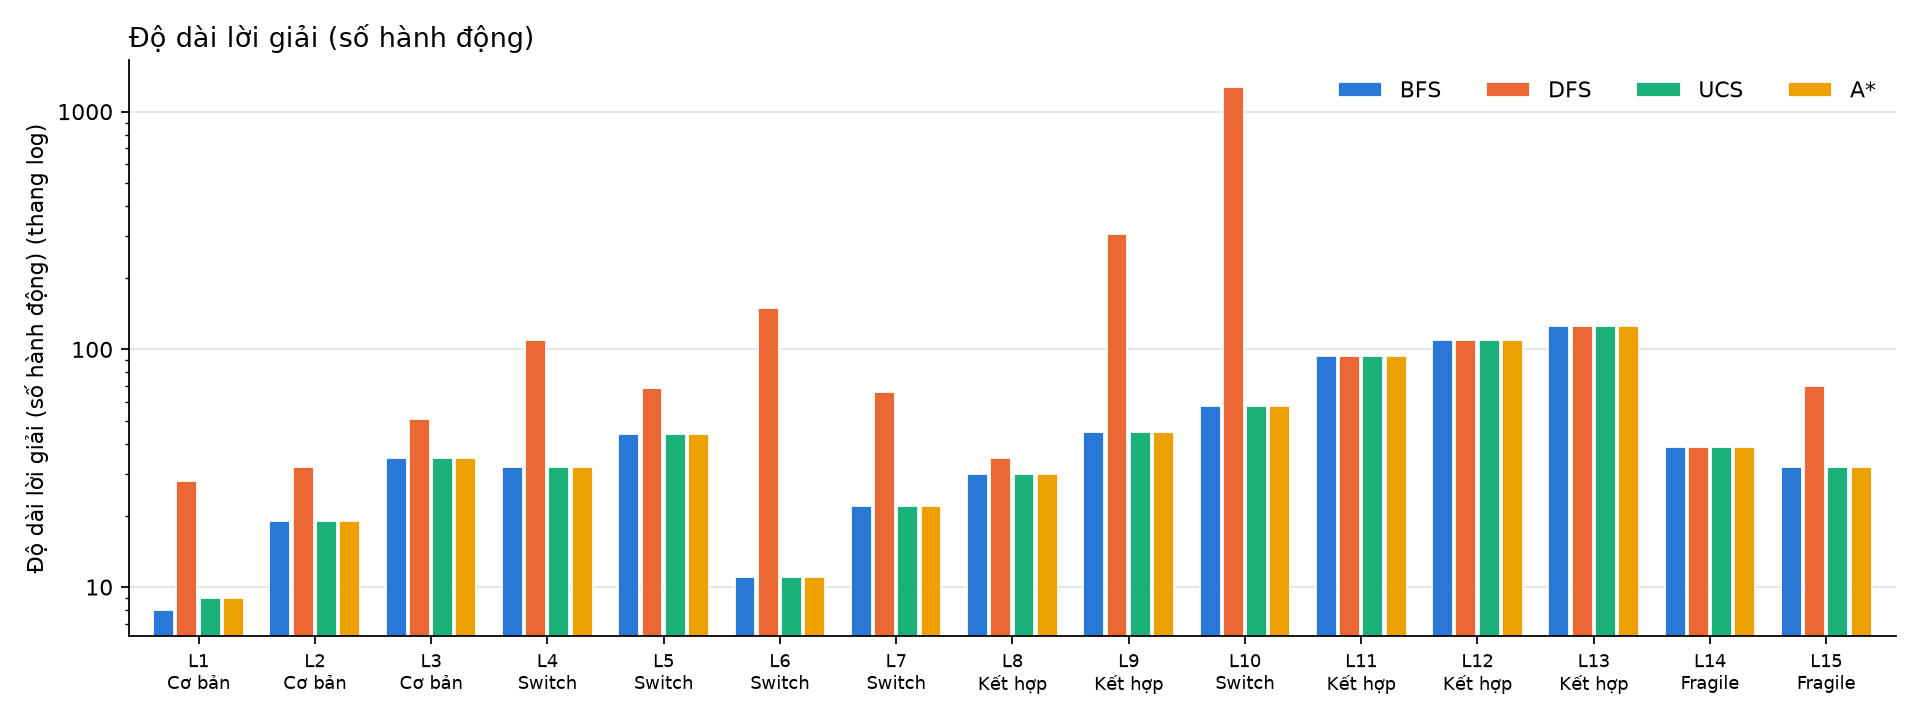
\includegraphics[width=1.0\linewidth]{figures/length.png}
\caption{So sánh độ dài lời giải trên 15 màn.}\end{figure}
\begin{figure}[H]\centering
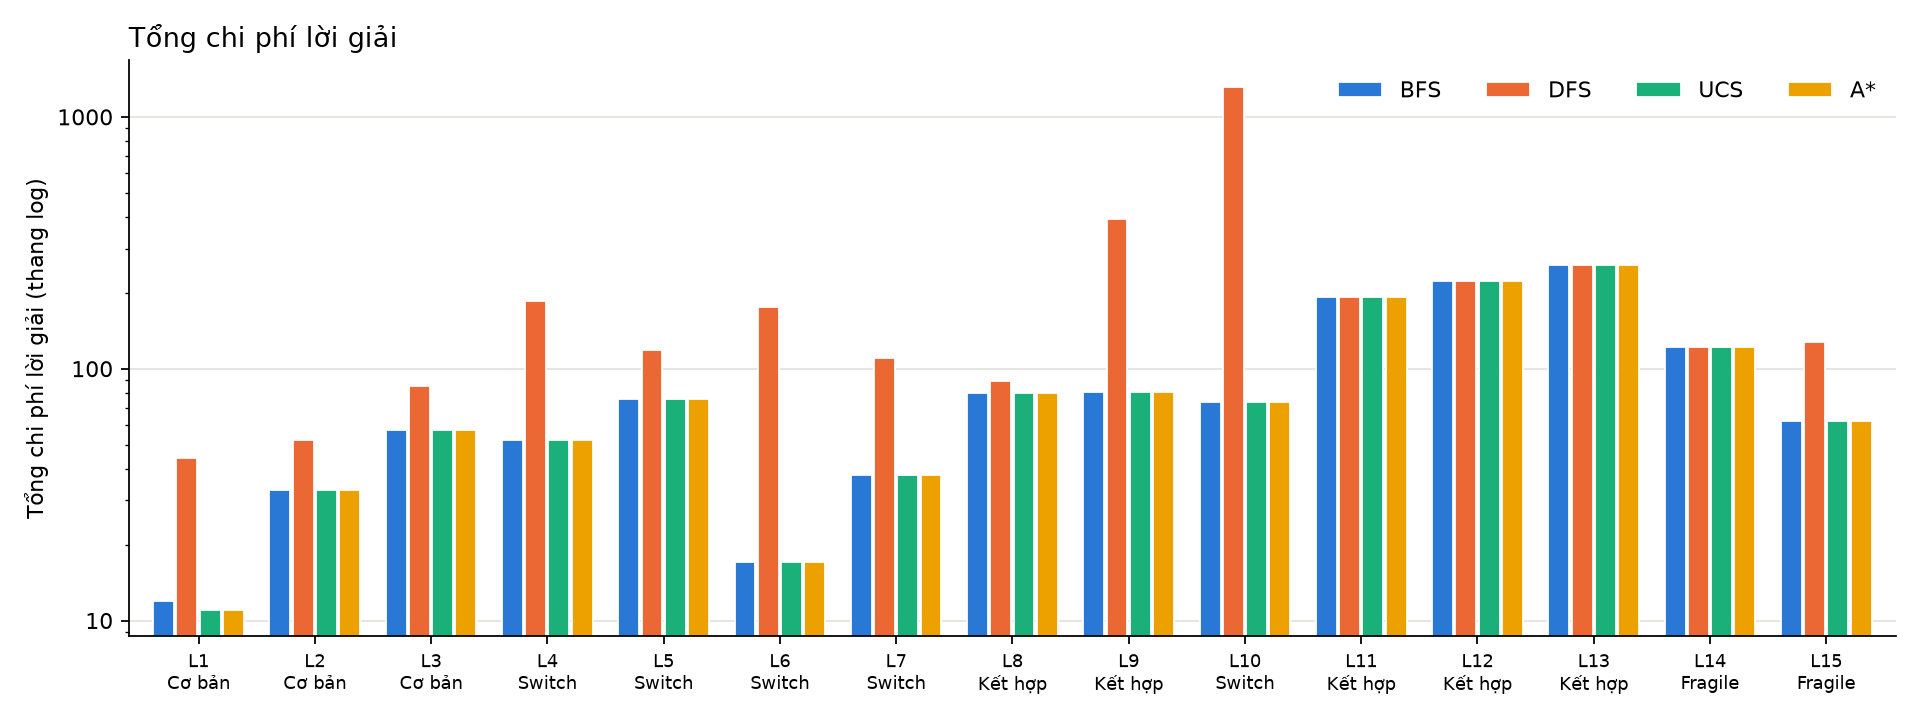
\includegraphics[width=1.0\linewidth]{figures/cost.png}
\caption{So sánh tổng chi phí lời giải theo quy tắc $1$--$2$--$4$.}\end{figure}
\clearpage
\begin{figure}[H]\centering
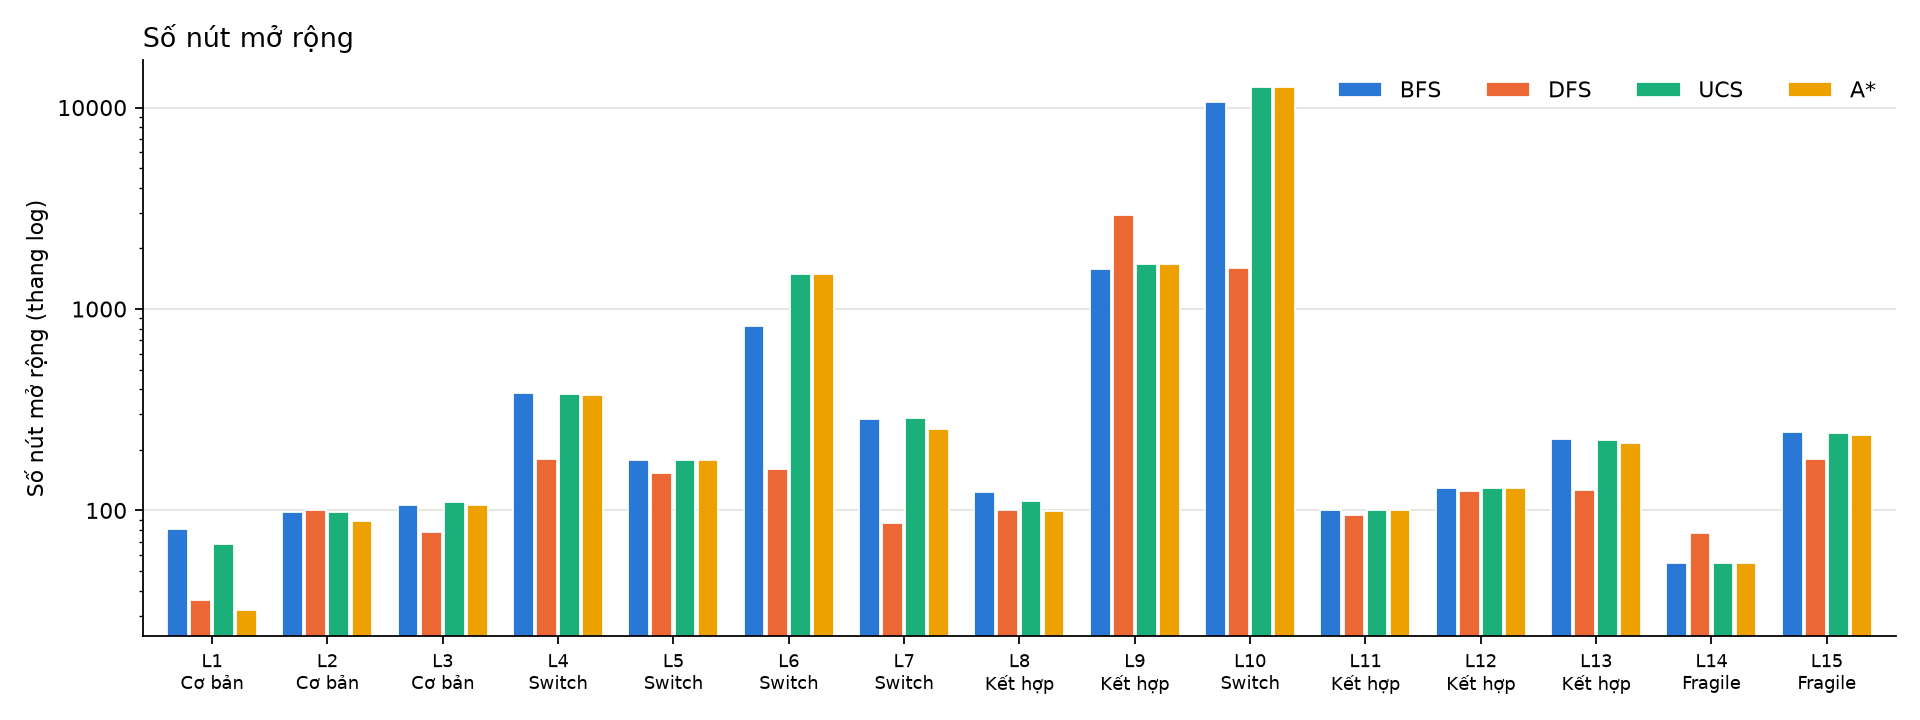
\includegraphics[width=1.0\linewidth]{figures/expanded.png}
\caption{So sánh số nút mở rộng trên từng màn.}\end{figure}
\begin{figure}[H]\centering
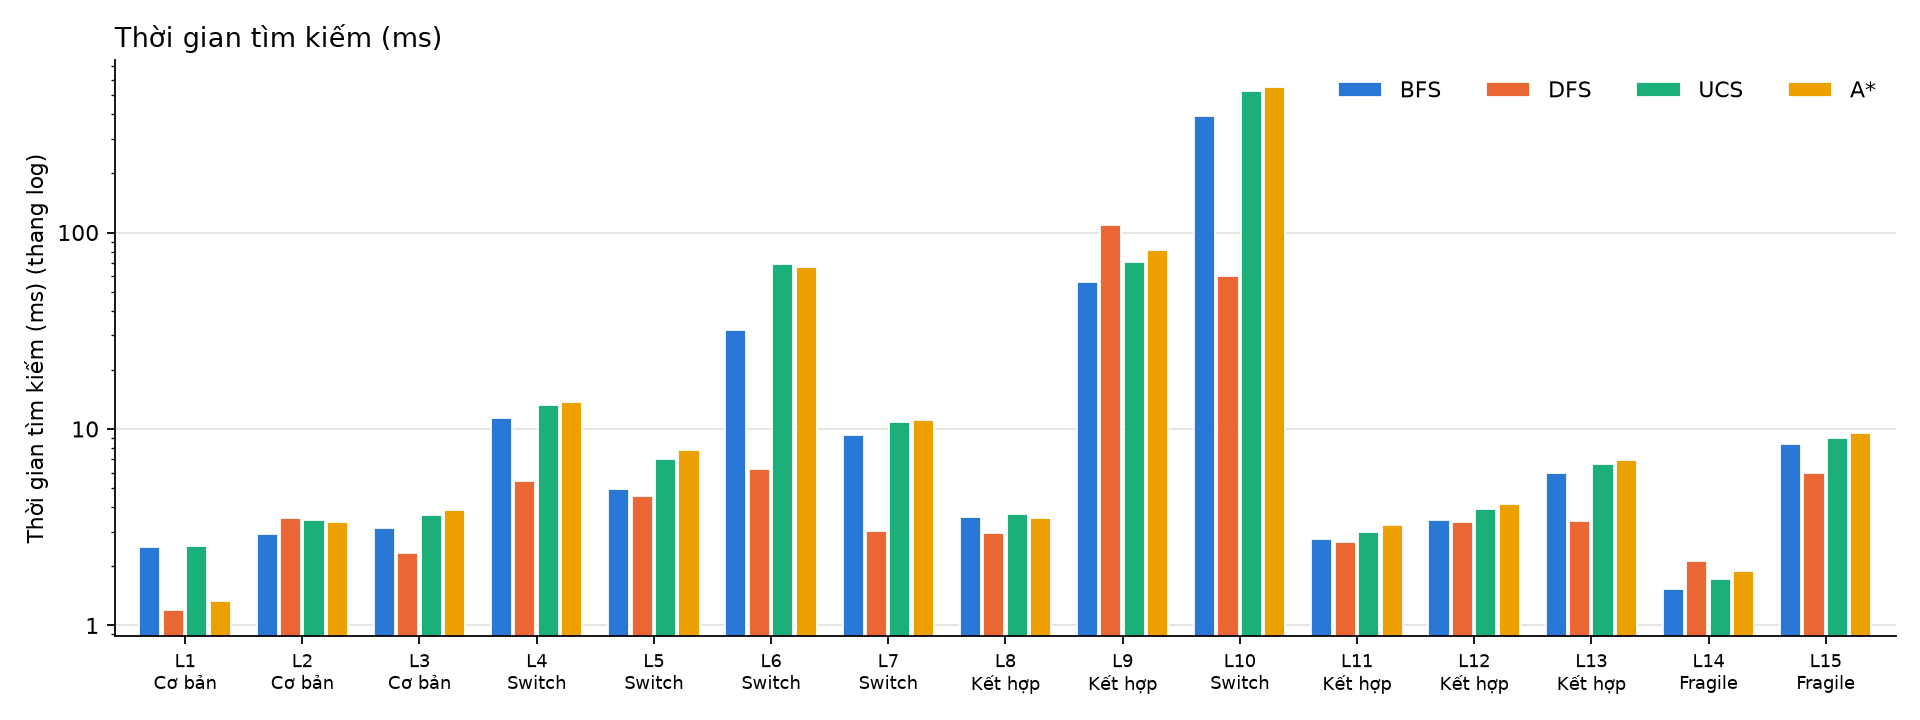
\includegraphics[width=1.0\linewidth]{figures/time.png}
\caption{Trung vị thời gian tìm kiếm theo từng màn, đơn vị ms.}
\caption*{Lưu ý: Trung vị thời gian có thể khác nhau giữa các lần đo tùy theo tình trạng hoạt động của máy.}\end{figure}
\clearpage
\begin{figure}[H]\centering
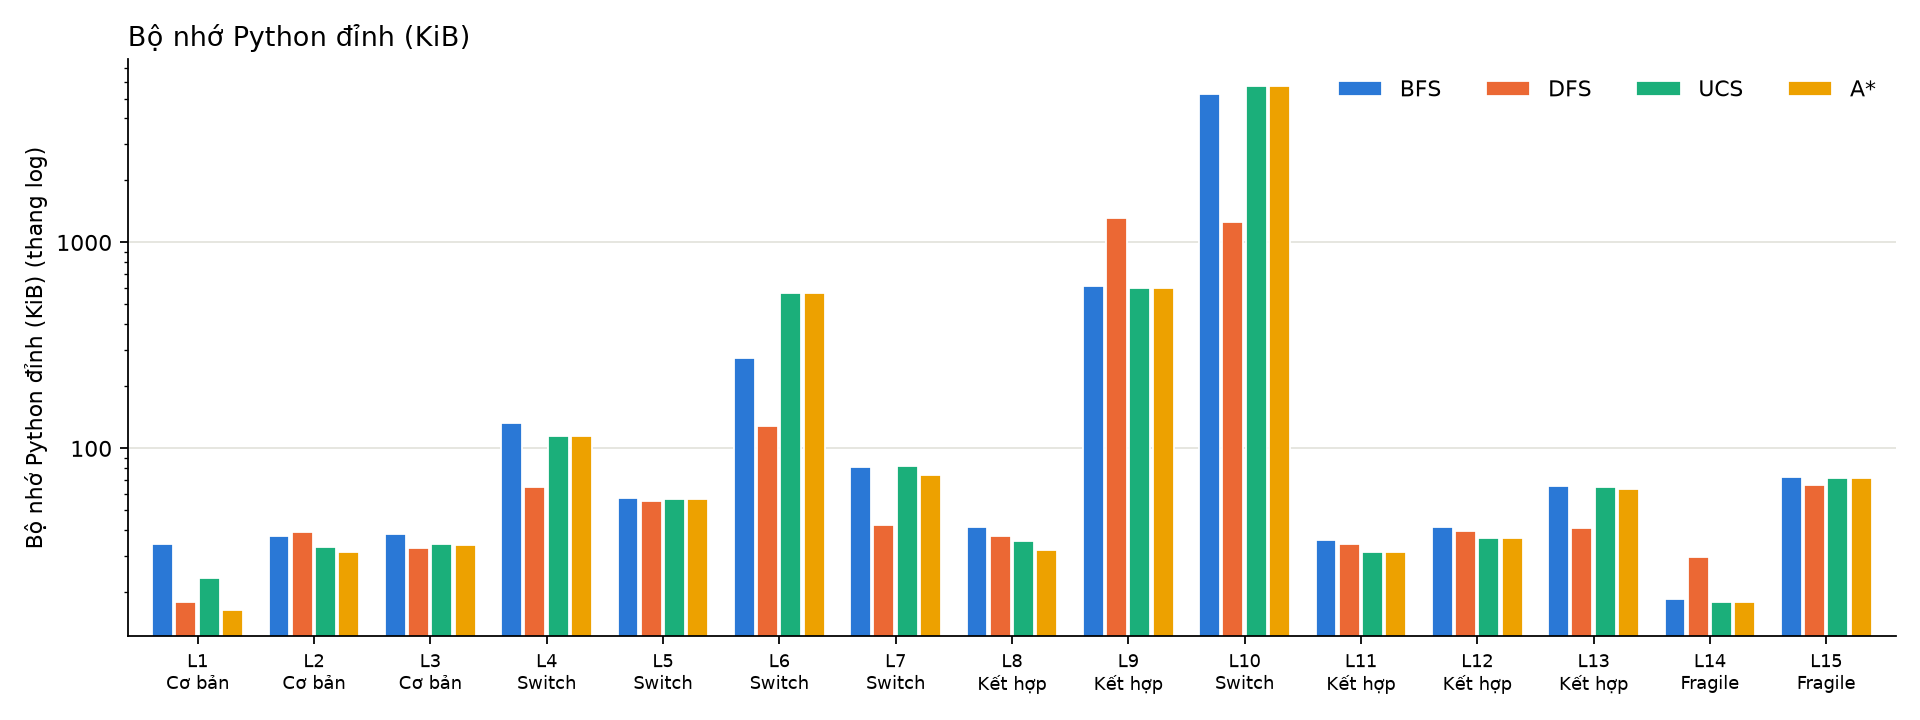
\includegraphics[width=1.0\linewidth]{figures/memory.png}
\caption{Bộ nhớ Python đỉnh theo từng màn, đơn vị KiB.}\end{figure}
\begin{figure}[H]\centering
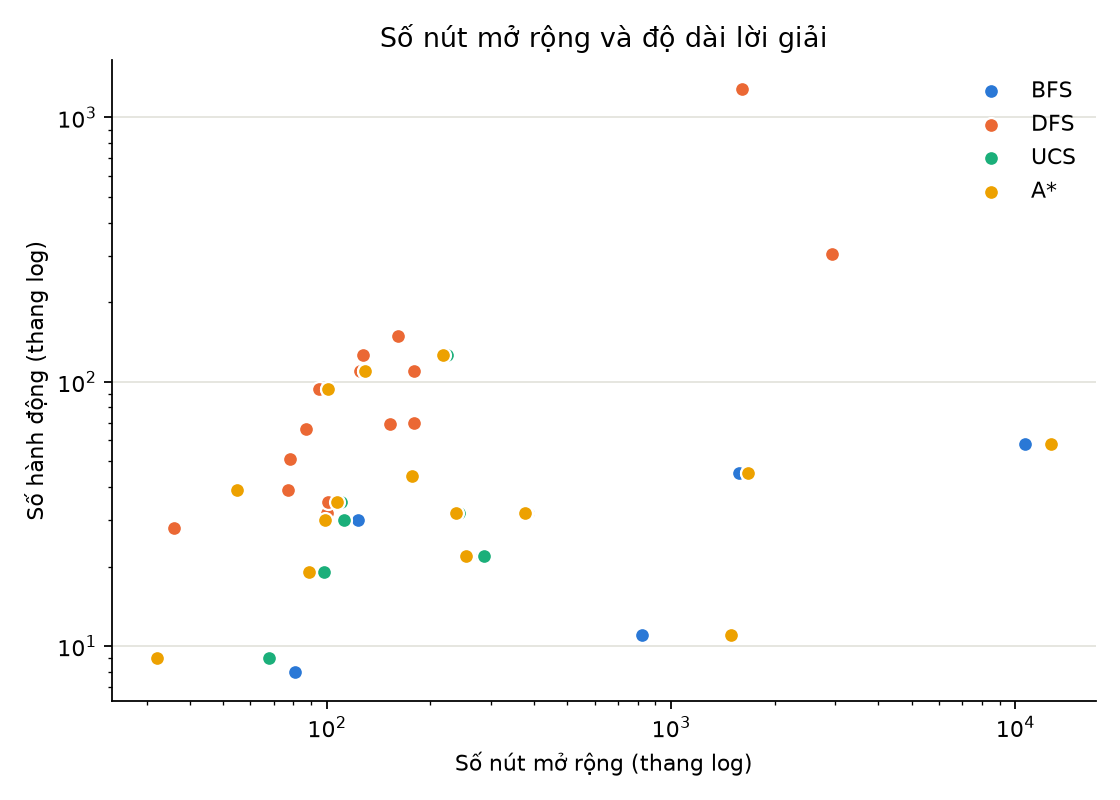
\includegraphics[width=0.80\linewidth]{figures/tradeoff.png}
\caption{Quan hệ giữa số nút mở rộng và số hành động của lời giải.}\end{figure}
\clearpage
\subsection{Phân tích kết quả}

\subsubsection{Độ dài và tổng chi phí lời giải}

Màn 1 minh họa rõ sự khác nhau giữa tối ưu số hành động và
tối ưu chi phí. BFS tìm lời giải gồm 8 hành động với Cost 12.
Trong khi đó, UCS và A* tìm lời giải gồm 9 hành động nhưng
Cost chỉ bằng 11. Như vậy, thêm một hành động giúp giảm
một đơn vị chi phí, tương đương khoảng $8.33\%$ so với
chi phí của đường BFS.

Kết quả này phù hợp với mục tiêu của các thuật toán:
BFS tối thiểu hóa số hành động, còn UCS và A* tối thiểu hóa
tổng trọng số. Vì vậy không thể kết luận UCS hoặc A* kém hơn
BFS chỉ vì đường đi có nhiều hành động hơn.

Ở 14 màn còn lại, BFS, UCS và A* có cùng Length và Cost.
Sự trùng số đo không chứng minh chuỗi hành động giống nhau
vì CSV không lưu đường đi cụ thể. Chi phí trung bình của BFS
là $91.733$, còn UCS và A* là $91.667$. Chênh lệch nhỏ do
bộ test hiện chỉ có màn 1 thể hiện khác biệt về chi phí
giữa các lời giải được trả về.

DFS có Length trung bình $170.667$ và Cost trung bình
$233.000$, cao hơn ba thuật toán còn lại. Trường hợp rõ nhất
là màn 10: DFS cần 1276 hành động với Cost 1320, trong khi
BFS, UCS và A* chỉ cần 58 hành động với Cost 74.
Đường đi DFS dài gấp $22$ lần và đắt khoảng $17.84$ lần.

Ở các màn 11, 12, 13 và 14, cả bốn thuật toán có cùng Length
và Cost. Tuy nhiên, chỉ từ kết quả này chưa thể khẳng định
mỗi màn chỉ có một đường tới đích.

\subsubsection{Hiệu quả của heuristic A*}

Ở màn 1 không có split, A* mở rộng 32 nút so với 68 nút
của UCS, giảm khoảng $52.94\%$. Thời gian tìm kiếm giảm từ
$2.546$ ms xuống $1.332$ ms, tương ứng khoảng $47.68\%$
trong lần đo này. Bộ nhớ cũng giảm từ $23.441$ KiB xuống
$16.402$ KiB.

Tuy nhiên, giảm số nút không luôn làm thời gian giảm.
Ở màn 7, A* mở 254 nút so với 286 nút của UCS, nhưng
thời gian là $11.145$ ms so với $10.854$ ms.
Ở màn 13, số nút giảm từ 224 xuống 217 nhưng thời gian
tăng từ $6.615$ ms lên $6.973$ ms.
Chi phí tính heuristic và biến động môi trường thực thi
là các khả năng giải thích; dữ liệu hiện tại chưa tách
riêng được ảnh hưởng của từng nguyên nhân.

Trên các màn split 6, 9 và 10, A* sử dụng $h=0$ nên có
chiến lược tương đương UCS. Expanded, Generated, Length
và Cost của hai thuật toán trùng nhau trên cả ba màn.
Chẳng hạn ở màn 10, cả UCS và A* đều mở rộng 12722 nút
và sinh 45981 successor.

Thời gian vẫn có thể khác dù thứ tự tìm kiếm tương đương.
Ở màn 10, UCS mất $527.138$ ms, còn A* mất $553.506$ ms.
Không xem đây là bằng chứng về hiệu quả định hướng
của heuristic vì heuristic trên màn này bằng không.

Trên toàn bộ bộ test, số nút trung bình của A* là
$1184.333$, so với $1191.600$ của UCS, chỉ giảm khoảng
$0.61\%$. Thời gian trung bình của A* là $51.509$ ms,
cao hơn UCS với $49.013$ ms. Vì vậy bộ số liệu này
không hỗ trợ kết luận A* luôn nhanh hơn UCS.

\subsubsection{BFS và UCS khi chi phí không đồng nhất}

Với trọng số $1$--$2$--$4$, thứ tự mở rộng của UCS không còn
nhất thiết giống BFS. BFS ưu tiên ít hành động từ điểm đầu,
còn UCS ưu tiên tổng chi phí đã đi nhỏ nhất.

Ở màn 6, BFS mở rộng 824 nút trong khi UCS mở rộng 1494 nút.
Ở màn 10, các giá trị tương ứng là 10671 và 12722.
UCS có thể phải khảo sát nhiều trạng thái đạt được bằng
các hành động rẻ trước khi lấy đích ra khỏi hàng đợi.
Vì vậy việc UCS mở nhiều nút hơn BFS không tự động cho thấy
thuật toán sai.

Trên toàn bộ bộ test, BFS có thời gian trung bình
$35.833$ ms và bộ nhớ trung bình $452.786$ KiB.
Hai giá trị này thấp hơn UCS, lần lượt là $49.013$ ms và
$503.263$ KiB. Đổi lại, UCS bảo đảm tối ưu tổng chi phí,
trong khi BFS bảo đảm tối ưu số hành động.
So sánh tài nguyên cần đi kèm mục tiêu tối ưu tương ứng.

\subsubsection{Đặc điểm của DFS}

DFS có thời gian trung bình thấp nhất trong lần thực nghiệm
này, bằng $14.392$ ms. Số nút và bộ nhớ trung bình cũng thấp
nhất, lần lượt là $402.400$ nút và $213.653$ KiB.
Tuy nhiên, kết quả đó đi kèm lời giải có thể dài và đắt hơn
đáng kể, như trường hợp màn 10.

Màn 9 thể hiện hiệu quả không ổn định của DFS.
DFS mở 2936 nút, dùng $1314.402$ KiB và mất $109.279$ ms;
BFS tương ứng chỉ mở 1578 nút, dùng $612.105$ KiB và mất
$56.011$ ms. DFS cũng mở nhiều nút hơn BFS ở màn 2 và 14.

Các kết quả này phù hợp với việc DFS phụ thuộc vào
thứ tự sinh successor và vị trí của đích trong nhánh
được duyệt trước. Không thể suy rộng từ thời gian trung bình
thấp nhất trên bộ test này thành kết luận DFS luôn nhanh nhất.

\subsubsection{Ảnh hưởng của bản đồ và bộ nhớ}

Màn 10 có thời gian tìm kiếm lớn nhất đối với BFS, UCS và A*. Riêng DFS mất nhiều thời gian nhất ở màn 9.
Đây cũng là màn dùng bộ nhớ lớn nhất đối với BFS, UCS và A*.
Với UCS, bộ nhớ đỉnh đạt $5779.180$ KiB, xấp xỉ $5.64$ MiB.
Riêng DFS dùng bộ nhớ lớn nhất ở màn 9 với $1314.402$ KiB,
cao hơn màn 10 với $1260.461$ KiB.

Đối với BFS, thời gian trung vị của riêng màn 10 chiếm
khoảng $72.50\%$ tổng thời gian trung vị trên 15 màn.
Do đó số trung bình toàn bộ bị ảnh hưởng mạnh bởi
một màn có không gian tìm kiếm lớn.

Ngược lại, màn 13 có lời giải dài 126 hành động, nhiều hơn
màn 10, nhưng UCS chỉ mở rộng 224 nút và mất $6.615$ ms.
Điều này cho thấy độ dài lời giải chưa đủ để mô tả
độ khó tìm kiếm.

Công tắc và cầu làm tăng số cấu hình động, còn split bổ sung
vị trí hai cube và cube chủ động vào trạng thái.
Tuy nhiên chỉ những tổ hợp thực sự tới được mới được khảo sát.
Hình dạng bản đồ và mức độ phân nhánh cũng ảnh hưởng
đến tài nguyên tiêu thụ.

Trong cài đặt của nhóm, cả BFS và DFS đều lưu
\texttt{visited} và \texttt{parents}.
BFS sử dụng danh sách với chỉ số đầu hàng đợi nên vẫn giữ
các phần tử đã lấy ra. UCS và A* sử dụng bảng chi phí cùng
heap có thể chứa các mục cũ. Vì vậy không thể suy ra
bộ nhớ đỉnh chỉ từ số nút mở rộng.

\subsection{Giới hạn của thực nghiệm}

Bộ dữ liệu gồm 15 màn đều được báo giải thành công.
Chưa có số liệu cho các màn vô nghiệm hoặc những cấu hình
biên chuyên biệt của luật game.

CSV chỉ lưu trung vị thời gian và một lượt đo bộ nhớ
cho mỗi cặp thuật toán/màn. Các thời gian thô và khoảng
biến thiên chưa được lưu nên chưa đủ cơ sở đánh giá
ý nghĩa thống kê của các chênh lệch nhỏ.

Kiểm tra replay xác nhận tính hợp lệ theo mô hình đã
cài đặt, không chứng minh mọi trường hợp của luật game
đều đúng. Đặc biệt, kết quả này không có nghĩa cơ chế
tự ghép ngay sau teleport đã được bổ sung; nhóm giữ nguyên
cơ chế kiểm tra ghép sau hành động di chuyển cube.

Trong phạm vi bộ test hiện tại, cả bốn thuật toán đều
trả lời giải hợp lệ theo mô hình. BFS cho số hành động
ít nhất; UCS và A* cho cùng chi phí, phù hợp với bảo đảm
tối ưu theo hàm chi phí đã chọn. DFS có tài nguyên trung bình
thấp hơn nhưng chất lượng lời giải có thể giảm đáng kể.
Khi thay đổi luật, hàm chi phí hoặc bộ màn, cần chạy lại
thực nghiệm trước khi sử dụng các kết luận trên.

\clearpage
\section{Kết luận và hướng phát triển}
Đồ án xây dựng trò chơi Bloxorz bằng Python với giao diện Ursina và bốn thuật toán BFS, DFS, UCS, A*. Trạng thái tìm kiếm bao gồm vị trí, tư thế khối, cấu hình cầu, vị trí hai khối đơn và quyền điều khiển khi tách. Các thuật toán dùng chung luật chuyển trạng thái, nhờ đó kết quả được so sánh trên cùng bài toán.

Trên bộ 15 màn, cả 60 kết quả đều có lời giải hợp lệ và chi phí khớp với phép tính lại dọc đường đi. BFS cho số hành động nhỏ nhất; UCS và A* có cùng chi phí trên tất cả các màn. Màn 1 thể hiện rõ khác biệt giữa hai mục tiêu: BFS đi 8 bước với chi phí 12, trong khi UCS và A* đi 9 bước với chi phí 11.

DFS đạt thời gian trung bình thấp nhất, nhưng chất lượng lời giải không ổn định. Ở màn 10, lời giải DFS dài gấp 22 lần lời giải BFS. Vì vậy, DFS phù hợp để tìm nhanh một lời giải khi thứ tự duyệt thuận lợi, nhưng không phù hợp nếu cần bảo đảm số bước hoặc tổng chi phí nhỏ nhất.

A* giảm số nút so với UCS ở một số màn không có split, rõ nhất là màn 1 với mức giảm khoảng 52.94\%. Trên các màn split 6, 9 và 10, heuristic bằng 0 nên chiến lược tìm kiếm tương đương UCS. Tổng hợp toàn bộ bộ test, A* chỉ giảm khoảng 0.61\% số nút mở rộng và có thời gian trung bình cao hơn UCS. Kết quả cho thấy lợi ích của A* phụ thuộc chất lượng heuristic và cấu trúc màn chơi.

Giới hạn chính của chương trình là heuristic chưa khai thác được teleport, STOP chưa hủy ngay vòng tìm kiếm và thao tác ghép khối chỉ được xét sau khi di chuyển một cube. Bộ thực nghiệm chưa bao gồm màn vô nghiệm, chưa lưu số đo thời gian thô và thông tin phần cứng, nên chưa đủ để suy rộng kết luận về hiệu năng sang các môi trường khác.

Hướng phát triển gồm bổ sung kiểm thử độc lập cho luật công tắc và tách ghép; tập trung hàm chi phí vào một mô-đun dùng chung; hỗ trợ tín hiệu hủy solver; xây dựng heuristic dựa trên bài toán nới lỏng có teleport. Bộ test cần được mở rộng bằng các màn có nhiều đường cạnh tranh về chi phí để đánh giá rõ hơn lợi ích của UCS và A*.

\clearpage
\phantomsection
\addcontentsline{toc}{section}{Tài liệu tham khảo}
\begin{thebibliography}{9}
\bibitem{de} Khoa Công nghệ Thông tin, Trường Đại học Khoa học Tự nhiên, ĐHQG-HCM. \textit{CSC14003 Introduction to Artificial Intelligence, Project 1: Bloxorz Solver} [Đề bài học phần], 8 trang.
\bibitem{reference-game} KhoaTranFitus. \textit{Bloxorz AI HCMUS} [Mã nguồn]. GitHub. Nguồn tham khảo cho phần core game và 10 màn được chọn trong bộ test. \url{https://github.com/KhoaTranFitus/Bloxorz_AI_HCMUS}.
\bibitem{template} lenbui. \textit{Report template} [Mẫu báo cáo LaTeX]. GitHub. \url{https://github.com/lenbui/report-template}.
\end{thebibliography}
\appendix
\section{Hướng dẫn chạy chương trình và tái lập thực nghiệm}
Mã nguồn hướng tới Python 3.13 theo tệp README. Tại thư mục \texttt{source}, tạo và kích hoạt môi trường ảo, cài các thư viện trong \texttt{requirements.txt}, sau đó chạy trò chơi:
\begin{lstlisting}[language=bash,numbers=none]
python -m pip install -r requirements.txt
python main.py
\end{lstlisting}
Phím mũi tên hoặc WASD dùng để di chuyển; Space đổi cube đang điều khiển; R khởi động lại màn; Esc trở về danh sách màn. Các nút BFS, DFS, UCS và A* gọi bộ giải từ trạng thái đầu; RESULTS mở bảng thống kê.

Để chạy thực nghiệm bốn thuật toán với năm lượt đo thời gian cho mỗi màn, dùng script có kiểm tra chi phí:
\begin{lstlisting}[language=bash,numbers=none]
python -m experiments.search_experiment --algos all \
  --runs 5 --out experiments/report_results
\end{lstlisting}
Có thể thêm \texttt{--no-plot} để chỉ xuất số liệu. Thư mục kết quả chứa CSV chi tiết theo màn, CSV trung bình theo nhóm và các biểu đồ. Tham số \texttt{--out} nên trỏ đến một thư mục mới khi cần giữ lại kết quả trước đó.

Khi tái lập, giữ nguyên các tệp \texttt{level1.json} đến \texttt{level15.json}, thứ tự sinh hành động và quy tắc chi phí. Ghi lại CPU, RAM, hệ điều hành, phiên bản Python, số lượt đo và phiên bản mã nguồn để so sánh các lần chạy. Thời gian có thể thay đổi giữa các môi trường; số bước, chi phí và bộ đếm nút cần được đối chiếu riêng với CSV.

\clearpage
\section{Liên kết mã nguồn và video demo đồ án}

\noindent\textbf{Mã nguồn GitHub:} \url{https://github.com/hohuunghiem/Fundamentals-of-Artificial-Intelligence}

\noindent Kho lưu trữ này chứa mã nguồn, các thư mục dữ liệu và kết quả thực nghiệm của đồ án Bloxorz Solver.

\vspace{5mm}
\noindent\textbf{Video demo:} \url{https://youtu.be/bJiol6gotSw}

\end{document}
